\documentclass[11pt]{article}
\usepackage{float}
\usepackage[utf8]{inputenc}
\usepackage[T1]{fontenc}
\usepackage{amsmath, amssymb, amsthm}
\usepackage[hidelinks]{hyperref}
\usepackage{listings}
\usepackage{xcolor}
\usepackage{graphicx}
\usepackage[UTF8]{ctex}

\renewcommand{\figurename}{Rysunek}
\renewcommand{\tablename}{Tabela}

\graphicspath{{./img}}

\definecolor{comment}{RGB}{0,128,0} % dark green
\definecolor{string}{RGB}{255,0,0}  % red
\definecolor{keyword}{RGB}{0,0,255} % blue
\lstset{language=C} 

\lstdefinestyle{mystyle}{
    commentstyle=\color{comment},
	stringstyle=\color{string},
	keywordstyle=\color{keyword},
	basicstyle=\footnotesize\ttfamily,
	numbers=left,
	numberstyle=\tiny,
	numbersep=5pt,
	frame=lines,
	breaklines=true,
	prebreak=\raisebox{0ex}[0ex][0ex]{\ensuremath{\hookleftarrow}},
	showstringspaces=false,
	upquote=true,
	tabsize=2,
}

\lstset{style=mystyle}


\title{Wbudy do budy}
\author{Dawid Gradowski (puckmoment na dc)}
\date{Luty 2025}
\begin{document}
\maketitle
\renewcommand\contentsname{Spis treści}
\tableofcontents
\newpage
\section{Prolog}
Notatki robione w oparciu o projekt, który robiłem sam na zajęciach (Licznik jak coś).

\begin{table}[H]
    \centering
    \label{tab:tab1}
    \begin{tabular}{ |c|c|c| }
        \hline
        \multicolumn{3}{|c|}{Komponenciki}\\
        \hline
        Płytka & LPC1768/9 & \href{https://dgradowski.github.io/Notes-page/docs/sem4/wbudowane/notatka/docs/Schemat%20ver%20B%20(z%20portem%20USB%20typu%20A).pdf}{Schemat} \\ 
        \hline
        Ekran OLED & Rodzaj & Intrukcja \\
        \hline
        Termometr & LM75 & \href{https://dgradowski.github.io/Notes-page/docs/sem4/wbudowane/notatka/docs/LM75.pdf}{Instrukcja} \\
        \hline  
    \end{tabular}
    \caption{Używane urządzenia z przydatnymi dokumentami}
\end{table}
\section{GPIO}
\subsection{Informacje ogólne}
\textbf{GPIO} (General Purpose Input/Output) jest interfejsem, który 
możemy wykorzystać zarówno jako wejście jak i wyjście. To jak zachowuje się 
ten interfejs zależne jest od stanu Enable Line. Jeśli stan Enable Line jest
1 to interfejs robi za wejście, a jeśli 0 to robi za wyjście.

Płytka LPC1768 ma 5 portów (oznaczone od 0 do 4) i każdemu z nich
odpowiadają 4 rejestry 32 bitowe. Rejestry te w pliku oraz w programie możemy
odnaleźć pod nazwami:
\begin{itemize}
    \item \textbf{FIOPIN} - odczytywanie wartości na pinach
    \item \textbf{FIOSET} - ustawianie wartości 1 na pinach (ustawionych na output)
    \item \textbf{FIOCLR} - zerowanie wartości na pinach (ustawionych na output)
    \item \textbf{FIODIR} - ustalanie kierunku pinu (0: wejście| 1: wyjście)
\end{itemize}
Oznaczenie FIO oznacza Fast Input/Output, czyli IO (Input/Output) tylko szybsze
(tak przeczytałem na forum to nie żart). Teraz trochę jak korzystać z tych rejestrów w praktyce.
Mimo, że rejestry są 32 bitowe w przykładzie będę operował na pierwszych 4 bitach
bo nie chce mi się tyle pisać.
Na początku uznajmy, że wszystkie bity w rejestrach są ustawione na LOW (czyli 0).
\begin{table}[H]
    \centering
    \begin{tabular}{|c|c|c|c|c|}
        \hline
        Rejestr & 3 & 2 & 1 & 0 \\ \hline
        FIOPIN & 0 & 0 & 0 & 0 \\ \hline
        FIOSET & 0 & 0 & 0 & 0 \\ \hline
        FIOCLR & 0 & 0 & 0 & 0 \\ \hline
        FIODIR & 0 & 0 & 0 & 0 \\ \hline
    \end{tabular}
\end{table}
Interfejs taki ma 32 piny i w tym momencie są ustawione na wejście. Urządzenie więc
nie może tym interfejsem wysyłać sygnału. Załóżmy, że jakieś urządzenie jest podłączone
do pinu oznaczonego numerem 3 i nadaje sygnał wysoki (1). Wtedy nasza tabelka będzie wyglądała tak:
\begin{table}[H]
    \centering
    \begin{tabular}{|c|c|c|c|c|}
        \hline
        Rejestr & 3 & 2 & 1 & 0 \\ \hline
        FIOPIN & 1 & 0 & 0 & 0 \\ \hline
        FIOSET & 0 & 0 & 0 & 0 \\ \hline
        FIOCLR & 0 & 0 & 0 & 0 \\ \hline
        FIODIR & 0 & 0 & 0 & 0 \\ \hline
    \end{tabular}
\end{table}
\newpage
Jako iż wszystkie bity w FIODIR są ustawione na 0, to żaden z naszych pinów nie jest
wyjściem więc nie możemy zmieniać wartości na pinach. Aby zmienić wartość na konkretnym bicie
możemu użyć następującej funkcji:

\begin{lstlisting}
void GPIO_SetDir(uint8_t port, uint32_t bitValue, uint8_t dir)
{
	LPC_GPIO_TypeDef *pGPIO = GPIO_GetPointer(port);

	if (pGPIO != NULL) {
		// Enable Output
		if (dir) {
			pGPIO->FIODIR |= bitValue;
		}
		// Enable Input
		else {
			pGPIO->FIODIR &= ~bitValue;
		}
	}
}
\end{lstlisting}
Jeśli chcielibyśmy na przykład używać pinu 2 jako wyjścia to wartość binarna
w rejestrze FIODIR musi wyglądać następująco $0100$ co jest równe 4 w dziesiętnym.
Z tą wiedzą wiemy, że bit ten możemy zmienić wywołująć funkcję na jeden z poniższych sposobów:

\begin{lstlisting}[language=c]
GPIO_SetDir(0, (1 << 2), 1); // preferowany
GPIO_SetDir(0, 0x4, 1);
GPIO_SetDir(0, 4, 1);
\end{lstlisting}
Po wywołaniu funkcji nasze rejestry będą wyglądały następująco:
\begin{table}[H]
    \centering
    \begin{tabular}{|c|c|c|c|c|}
        \hline
        Rejestr & 3 & 2 & 1 & 0 \\ \hline
        FIOPIN & 1 & 0 & 0 & 0 \\ \hline
        FIOSET & 0 & 0 & 0 & 0 \\ \hline
        FIOCLR & 0 & 0 & 0 & 0 \\ \hline
        FIODIR & 0 & 1 & 0 & 0 \\ \hline
    \end{tabular}
\end{table}
Teraz możemy zmienić wartość bitu 2 w rejestrze FIOPIN, nie możemy tego jednak zrobić
bezpośrednio. Aby zmienić wartość na pinie oznaczonym numerem 2 naszego interfejsu
musimy wykorzystać rejestry \textbf{FIOSET} i \textbf{FIOCLR}. Aby zmienić wartość
w tych 2 rejestrach możemy wykorzystać poniższe 2 funkcje:
\begin{lstlisting}[language=c]
void GPIO_SetValue(uint8_t portNum, uint32_t bitValue)
{
    LPC_GPIO_TypeDef *pGPIO = GPIO_GetPointer(portNum);

    if (pGPIO != NULL) {
        pGPIO->FIOSET = bitValue;
    }
}

void GPIO_ClearValue(uint8_t portNum, uint32_t bitValue)
{
	LPC_GPIO_TypeDef *pGPIO = GPIO_GetPointer(portNum);

	if (pGPIO != NULL) {
		pGPIO->FIOCLR = bitValue;
	}
}
\end{lstlisting}
Te 2 rejestry i funkcje działają w sposób bardzo podobny. Obydwa odpowiadają za zmiane
wartości w rejestrze FIOPIN. FIOSET ustawia wartość na 1, FIOCLR ustawia wartość na 0.
Obydwa rejestry po zmianie bitu w rejestrze FIOPIN od razu są zerowane. A więc by zmieniać
wartość pinu 2, trzeba wywołać metodę w taki sposób:
\begin{lstlisting}[language=c]
GPIO_SetValue(0, (1 << 2)); // preferowany
GPIO_SetValue(0, 0x4);
GPIO_SetValue(0, 4);
\end{lstlisting}
\newpage
Po wykonaniu tej funkcji wartości w rejestrach będą wyglądały następująco:
\begin{table}[H]
    \centering
    \begin{tabular}{|c|c|c|c|c|}
        \hline
        Rejestr & 3 & 2 & 1 & 0 \\ \hline
        FIOPIN & 1 & 0 & 0 & 0 \\ \hline
        FIOSET & 0 & 1 & 0 & 0 \\ \hline
        FIOCLR & 0 & 0 & 0 & 0 \\ \hline
        FIODIR & 0 & 1 & 0 & 0 \\ \hline
    \end{tabular}
\end{table}
I od razu zostanie zmienione na
\begin{table}[H]
    \centering
    \begin{tabular}{|c|c|c|c|c|}
        \hline
        Rejestr & 3 & 2 & 1 & 0 \\ \hline
        FIOPIN & 1 & 1 & 0 & 0 \\ \hline
        FIOSET & 0 & 0 & 0 & 0 \\ \hline
        FIOCLR & 0 & 0 & 0 & 0 \\ \hline
        FIODIR & 0 & 1 & 0 & 0 \\ \hline
    \end{tabular}
\end{table}
Wartość pinu zostanie zmieniona praktycznie natychmiast, według czatu GPT zazwyczaj w 1 lub 2
cyklach CPU, dlatego od razu po zmianie można odczytywać wartość w rejestrze FIOPIN oraz
nie ma sensu odczytywać wartości z rejestrów FIOSET i FIOCLR bo w większości przypadków
będą one równe 0. Metoda FIOCLR działa w ten sam sposób więc nie będę jej tłumaczył.
Zarówno FIOSET jak i FIOCLR nie zadziałają na piny, dla których odpowiadające im wartości
w rejestrze FIODIR są równe 0.
\newpage
Aby odczytać wartości z rejestru FIOPIN należy użyć następującej funkcji:
\begin{lstlisting}[language=c]
uint32_t GPIO_ReadValue(uint8_t portNum)
{
	LPC_GPIO_TypeDef *pGPIO = GPIO_GetPointer(portNum);

	if (pGPIO != NULL) {
		return pGPIO->FIOPIN;
	}

	return (0);
}
\end{lstlisting}
Dana funkcja odczytuje jednak całą wartość rejestru a nie pojedynczego bitu.
Jęśli chcemy napisać warunek zależny od tego czy mamy na bicie 3 wartość niską bądź
wysoką, to możemy to napisać na parę sposobów:

\begin{lstlisting}[language=c]
// preferowane
if if ((GPIO_ReadValue(0) & (1 << 3)) == 0) {
    // niski sygnal
} else {
    // wysoki sygnal
}

if (((GPIO_ReadValue(0) >> 3) & 0x01) == 0) {
    // niski sygnal
} else {
    // wysoki sygnal
}

if if ((GPIO_ReadValue(0) & 8) == 0) {
    // niski sygnal
} else {
    // wysoki sygnal
}
\end{lstlisting}
\subsection{Guziczki}
W poprzedniej sekcji wytłumaczyłem jak operować na rejestrach. Teraz czas na
użycie tej wiedzy w praktyce. W przypadku płytki LPC1768 mamy 3 zwykłe przyciski 
(2 z nich mają swoje przeznaczenie w samym działaniu płytki i nie powinniśmy 
zmieniać ich zastosowania (Wakeup i Reset))
i joystick, który wysyła sygnał na 5 różnych pinów (4 strony + wciśnięcie). W 
\hyperref[tab:tab1]{schemacie płytki zamieszczonym w tabeli 1} na stronie 6 podpisanej
jako Direct Digital IO peripherals. Nasz przycisk, który możemy wykorzystać wygląda 
w schemacie następująco:

\begin{figure}[H]
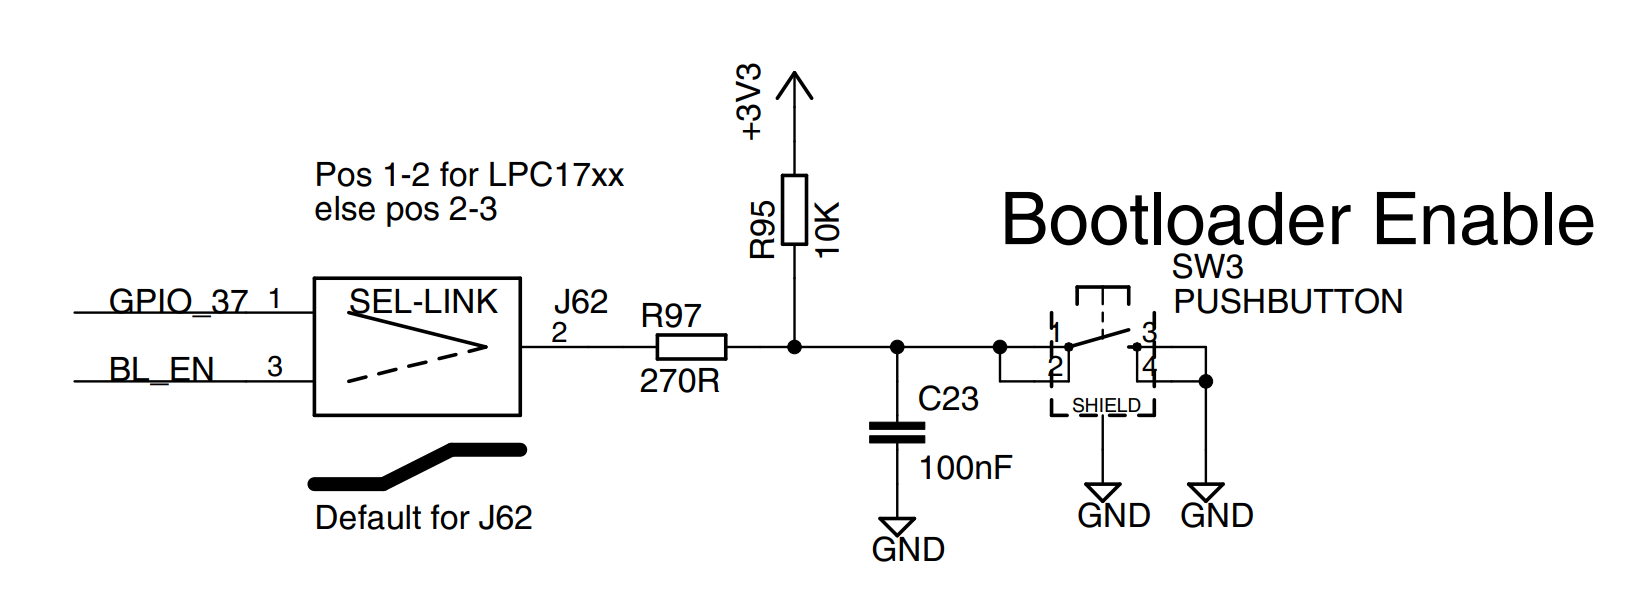
\includegraphics[width=\textwidth]{GPIO_btn.png}
\caption{Schemat przycisku SW3/Bootloader Enable}
\end{figure}

Wiemy, który przycisk chcemy wykorzystać patrząc na schemat. Jak teraz znaleźć go na
samej płytce? Wszystkie przyciski są bezpośrednio podpisane na płytce, więc musimy znaleźć
słowo klucz obok przycisku. Te słowa to SW3, GPIO\textunderscore 37 lub BL\textunderscore EN.

Jeśli widzimy przycisk na płytce i jesteśmy w gotowości by go przycisnąć to pozostało
nam tylko zaprogramować funkcjonalności, ale by to zrobić potrzebny jest nam adres
rejestru na który wpływa ten przycisk. Aby to odkryć znów będzie potrzebny schemat
płytki z \hyperref[tab:tab1]{tabeli 1} tylko tym razem strona 2. Na stronie drugiej
odszukujemy \textbf{BL\textunderscore EN} albo \textbf{GPIO\textunderscore 37}.
Akurat obydwa te oznaczenia są po lewej stronie więc na tej samej wysokości szukamy
komórki tabeli w kolumnie opisanej nazwą naszej płytki. Na tej samej wysokości co 
oznaczenie BL\textunderscore EN jest komórka w której mamy napisane \textbf{P0.4}.
Rozbijmy sobie to oznaczenie:
\begin{itemize}
    \item \textbf{P0} - port 0 (numerowany od 0)
    \item \textbf{4} - pin 4 (numerowany od 0)
\end{itemize}
GPIO\textunderscore 37 wskazuje też inny adres ale szczerze to nie sprawdzałem czy 
przycisk też zmienia pin na tym adresie, a jeśli nie to dlaczego ale chuj w to.

Mamy już w zasięgu palca nasz przycisk gotowy do wciśnięcia, znamy już adres na który
dany przycisk wpływa, pozostało tylko zaprogramować jakąś funkcjonalność. 
Przyciski jeśli chodzi o nadawany sygnał są bardzo nieintuicyjne, ponieważ niewciśnięty
przycisk daje na wyjściu 1, a wciśnięty daje 0. 

W instrukcji warunkowej możemy przycisków użyć w następujący sposób.
\begin{lstlisting}
if ((GPIO_ReadValue(0) & (1 << 4)) == 0) {
    // przycisk wcisniety
} else {
    // przycisk nie wcisniety
}

if ((GPIO_ReadValue(0) & (1 << 4)) > 0) {
    // przycisk nie wcisniety
} else {
    // przycisk wcisniety
}
\end{lstlisting}
\textbf{UWAGA. Trzeba pamiętać, że wartość FIODIR odpowiadający pinowi na który
przycisk nadaje musi być ustawiona na 0. W innym wypadku pin nie będzie odbierał sygnału
z przycisku.}

\section{SPI}
\subsection{Informacje ogólne}
To o czym będę mówił jest dość spoko wytłumaczone w tym filmiku: \href{https://www.youtube.com/watch?v=0nVNwozXsIc&ab_channel=Rohde%26Schwarz}{LINK}.


SPI jest szeregowym interfejsem urządzeń peryferyjnych. Jest nazywany
protokołem master-slave. Za mastera uznaje się kontroler i jest on zawsze
jeden a funkcję slave pełni urządzenie peryfejryne, które musi być jedno bądź więcej.
\subsubsection{Połączenia}
Każde połączenie między masterem a slavem ma do 4 kabli, które są odpowiedzialne
za 4 różne sygnały logiczne (logic signals). Te sygnały to:
\begin{itemize}
    \item {
        \textbf{CS / SS} (Chip Select lub Slave Select) - odpowiada za wybór 
        urządzenia do komunikacji
    }
    \item {
        \textbf{SCLK} (Synchronous Clock) - odpowiada za synchronizacje i timing(?)
    }
    \item {
        \textbf{MOSI} (Master Out Slave In) - dane przesyłane
        przez mastera
    }
    \item {
        \textbf{MISO} (Master In Slave Out) - dane odbierane przez
        mastera (opcjonalne)
    }
\end{itemize}
Z tego filmiku też kradne obrazki więc no. A więc wszystkie te sygnały są używane do komuniakcji.
\begin{figure}[H]
    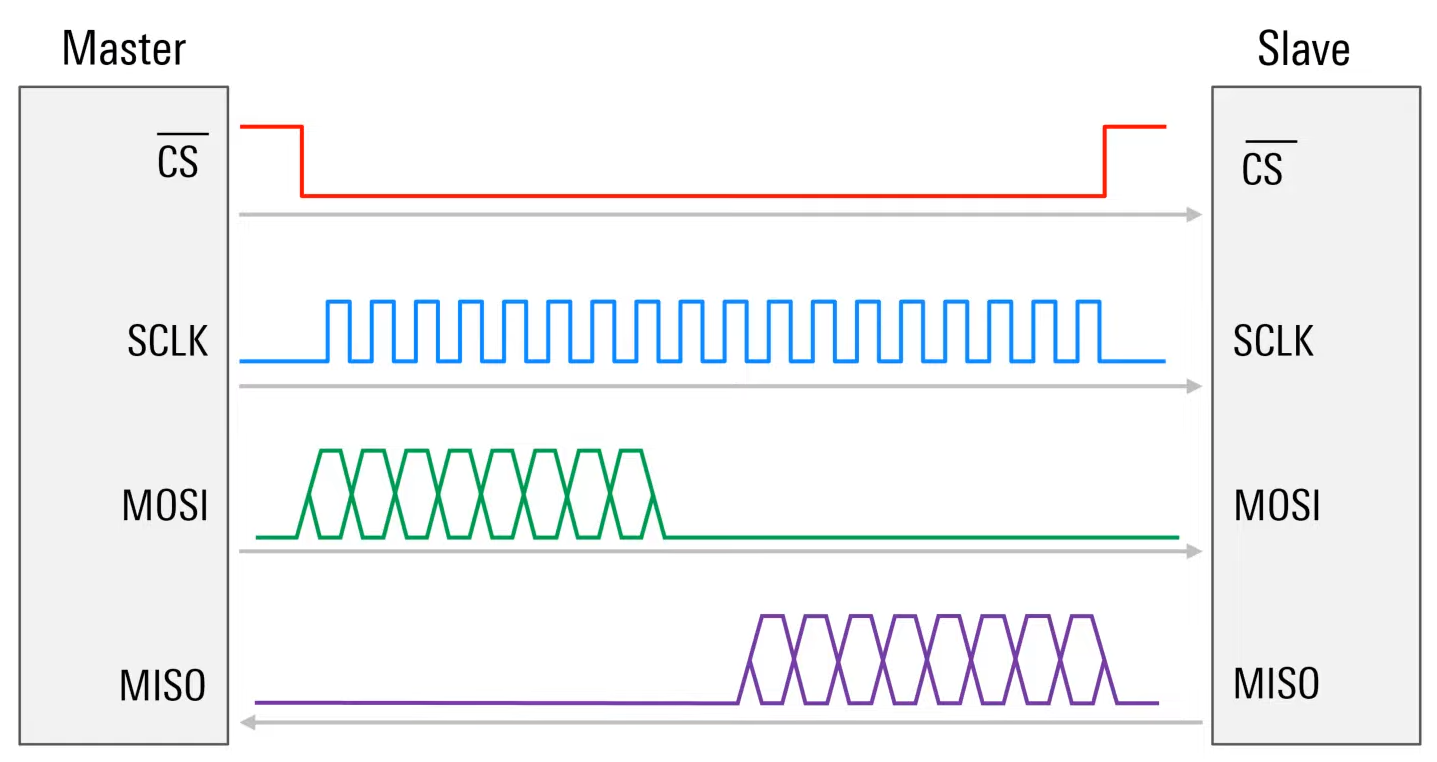
\includegraphics[width=\textwidth]{SPI_communication.png}
    \caption{Schemat komunikacji Master-Slave w interfejsie SPI}
\end{figure}
Etapy komunikacji w tym interfejsie wyglądają następująco:
\begin{enumerate}
    \item {
        Na lini CS następuje zmiana sygnału z wysokiego na niski. Oznacza to, że slave
        do którego trafia niski sygnał, będzie tym z którym master będzie się komunikował.
    }
    \item {
        Na lini SCLK wysyłany sygnał zmienia się z wysokiego na niski i z powrotem, by ustalić
        częstotliwość wysyłanych i odbieranych sygnałów z lini MOSI i MISO.
    }
    \item {
        Master wysyła sygnały niskie i wysokie za pomocą połączenia MOSI, a slave odsyła sygnał
        za pomocą połączenia MISO.
    }
    \item {
        Po zakończonej komunikacji sygnał na lini CS wraca do stanu wysokiego.
    }
\end{enumerate}

\subsubsection{SPI Modes}
SPI może pracować w 4 różnych trybach, zależnych od CPOL (clock polarity) i
CPHA (clock phase).

CPOL (clock polarity) oznacza czy na linii SCLK jest domyślnie stan niski czy wysoki
jak nie są wysyłane pakiety. Gdy CPOL jest równy 0 domyślną wartością jest wartość 0 (LOW),
a gdy CPOL jest równy 1 to domyślną wartością jest wartość 1.

CPHA (clock phase) oznacza czy dane są próbkowane gdy stan przechodzi z domyślnego na odwrotny (leading / first phase)
lub z odwrotnego na domyślny (trailing / second phase). Jeśli CPHA jest ustawione na 0 to dane
są próbkowane w fazie pierwszej, a jeśli 1 to w fazie drugiej.

Wszystkie te własności mogą być opisane jako SPI mode według wzoru poniższej tabelki:
\begin{table}[H]
    \centering
    \begin{tabular}{|c|c|c|}
        \hline
        SPI Mode & CPOL & CPHA \\
        \hline
        0 & 0 & 0 \\ \hline
        1 & 0 & 1 \\ \hline
        2 & 1 & 0 \\ \hline 
        0 & 1 & 1 \\
        \hline
    \end{tabular}
\end{table}
Najczęściej stosowanym trybem jest tryb 0.

\subsubsection{Łączenie wielu slave'ów}
Wiele slave'ów może być podłączonych do jednego mastera na 2 różne sposoby.
\begin{enumerate}
    \item {
        \textbf{Independend Slaves} - komunikacja z każdym urządzeniem podrzędnym 
        może przebiegać niezależnie od innych urządzeń. Plus jest taki, że jest dość 
        prosta w założeniu i na pewno taki sposób jest wspierany przez urządzenia podrzędne.
        Minus jest taki, że nie jest to dobrze skalowalne się rozwiązanie bo każde dodatkowe
        urządzenie potrzebuje dodatkowego połączenia CS.
        \begin{figure}[H]
            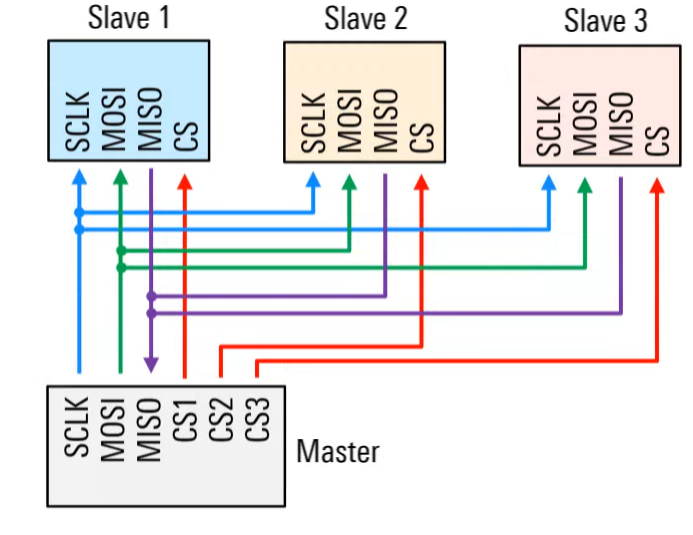
\includegraphics[width=\textwidth]{SPI_independent_slaves.png}
            \caption{Schemat komunikacji Independend Slaves}
        \end{figure}
    }
    \item {
        \textbf{Cooperative Slaves / Daisy Chain} - komunikacja z wszystkimi urządzeniami
        jest zależna od pozostałych urządzeń. Jeden sygnał CS mastera jest nadawany
        na wszystkie slave'y. Sygnał MISO wychodzący z urządzeń podrzędnych
        jest przekazywany do ścieżki MOSI kolejnego urządzenia podrzędnego, dopiero
        sygnał z ostatniego urządzenia podrzędnego trafia to MISO mastera. Plusem jest to,
        że skalowalność tego rozwiązania jest bardzo dobra (jedna ścieżka CS niezależnie od
        ilości urządzeń podrzędnych). Minus jest taki, że tego typu komunikacja jest bardzo
        skomplikowana i nie wszystkie urządzenia są z tym kompatybilne.
        \begin{figure}[H]
            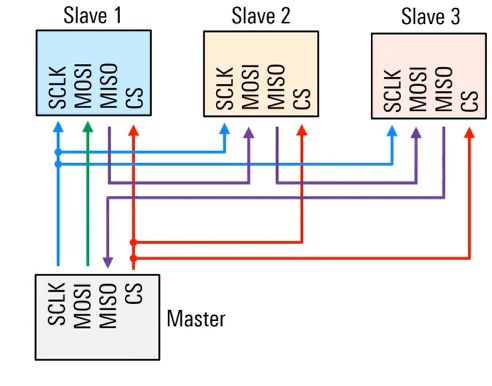
\includegraphics[width=\textwidth]{SPI_cooperative_slaves.png}
            \caption{Schemat komunikacji Cooperative Slaves}
        \end{figure}
    } 
\end{enumerate}

\subsection{Wyświetlacz}
Jeśli wierzyć skryptowi to wymiary ekranu na płytce LPC1768 to \textbf{96x64 pikseli},
ale sam kotroler może obsłużyć rozdzielczość do 132x64. Z tego co mówi chatGPT 
większość wyświetlaczy może wykorzystywać zarówno I$^2$C jak i SPI. Nasza płytka 
również może obsłużyć wyświetlacz za pomocą SPI oraz I$^2$C i widać to na schemacie znajdującym
się w \hyperref[tab:tab1]{tabeli 1}.
\begin{figure}[H]
    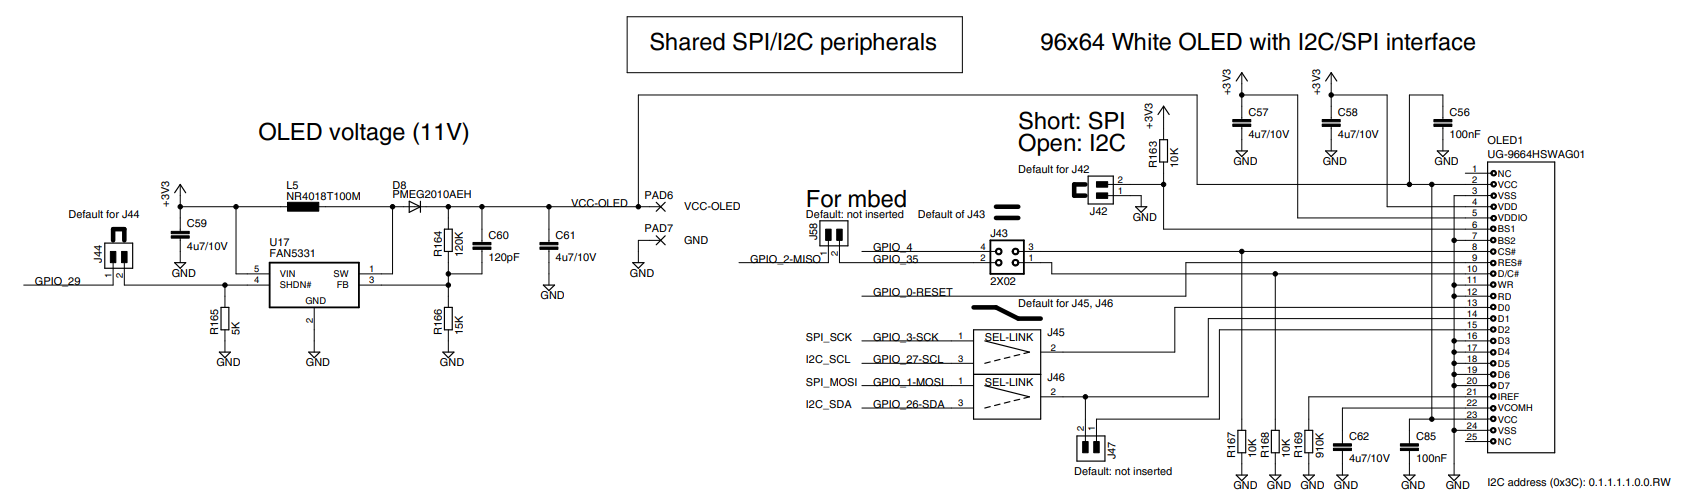
\includegraphics[width=\textwidth]{OLED.png}
    \caption{Schemat OLED}
\end{figure}
Teksty na rysunku są dość małe, ale to co najważniejsze wytłumaczę. Patrząc na ten
schemat oraz na samą płytkę możemy wywnioskować z jakiego interfejsu korzysta nasza 
płytka do komunikacji z wyświetlaczem. Jeden z większych tekstów na rysunku mówi:\newline
Short: SPI \newline
Open: I2C \newline
Co oznacza mniej więcej tyle, że jak zwarte (short) to używamy SPI, a jak jest 
otwarte to I$^2$C. Informacja ta odnosi się do punktu nazywanego jumper, który 
akurat w naszym przypadku jest oznaczony jako J42. Najprawdopodobniej są to jakieś 2
wystające piny, które można połączyć zworką.
Biblioteka, która była w przykładowych projektach i odpowiada za komunikacje z 
wyświetlaczem oled nazywa się oled.c. Jak ktoś chce dogłębnie poznać możliwości
biblioteki to niech sobie tam zajrzy, ja opiszę tylko to z czego korzystam sam.
Biblioteka ta może obsłużyć zarówno komunikacje przez SPI jak i I$^2$C. \newline
Poniższa linijka sugeruje, że używanym połączeniem jest SPI.
\begin{lstlisting}
//#define OLED_USE_I2C
\end{lstlisting}
Jeśli bardzo chcesz użyć interfejsu I$^2$C musisz odkomentować tą linijkę.

\subsubsection{Główna funckja zmieniająca konkretny pixel}
Główną funckją do zmiany koloru jednego pixela na ekranie oled jest funckja oled\textunderscore putPixel
z pliku oled.c. Funkcja ta jest zbyt długa bym ją zamieszczał ją tu w całości ciągiem więc omówie ją
w częściach. Zanim zaczniemy używać funkcji olde\textunderscore putPixel, musimy wywołać funkcję
oled\textunderscore init.
\begin{lstlisting}
void oled_init (void)
{
    int i = 0;

    //GPIO_SetDir(PORT0, 0, 1);
    GPIO_SetDir(2, (1<<1), 1);
    GPIO_SetDir(2, (1<<7), 1);
    GPIO_SetDir(0, (1<<6), 1);

    /* make sure power is off */
    GPIO_ClearValue( 2, (1<<1) );

    OLED_CS_OFF();

    runInitSequence();

    memset(shadowFB, 0, SHADOW_FB_SIZE);

    /* small delay before turning on power */
    for (i = 0; i < 0xffff; i++);

     /* power on */
    GPIO_SetValue( 2, (1<<1) );
}
\end{lstlisting}

\subsection{Zapis na kartę pamięci}

\section{I$^2$C}
\subsection{Czujnik natężenia światła}
\subsection{Termometr}
W przypadku termomemetru LM75 adres jest ustalany następująco:
\begin{center}
    \begin{tabular}{|c|c|c|c|c|c|c|}
        \hline
         & & & & $A_2$ & $A_1$ & $A_0$\\
        \hline
        1& 0& 0& 1& X & X & X\\
        \hline
    \end{tabular}
\end{center}
Pierwsze 4 bity są odczytane z instrukcji. Bity oznaczone $A_x$ są ustalane
zależnie od termometra na podstawie lutowania. Jeśli $A_x$ jest przylutowany
do gruntu (ground) to w adresie mamy 0, a jeśli do $+V_S$ to 1.
\section{RTC}
\end{document}